\documentclass[10pt,a4paper]{article}

% ---------- Packages ----------
\usepackage[utf8]{inputenc}
\usepackage[T1]{fontenc}
\usepackage[english]{babel}
\usepackage[a4paper,margin=1.7cm]{geometry}
\usepackage{graphicx}
\usepackage{booktabs}
\usepackage{float}
\usepackage{hyperref}
\usepackage{xcolor}
\usepackage{enumitem}
\usepackage{titlesec}

% ---------- Formatting ----------
\definecolor{navy}{RGB}{25,48,75}
\definecolor{teal}{RGB}{0,125,135}

\hypersetup{
    colorlinks=true,
    linkcolor=navy,
    urlcolor=teal
}

\titleformat{\section}
  {\large\bfseries\color{navy}}{\thesection}{0.6em}{}

\titleformat{\subsection}
  {\normalsize\bfseries\color{teal}}{\thesubsection}{0.6em}{}

\setlength{\parindent}{0pt}
\setlength{\parskip}{4pt}
\setlist{nosep,leftmargin=*}

% ---------- Document ----------
\begin{document}

% ================= PAGE 1 =================

\begin{center}
    {\large\bfseries UNIVERSITÉ CLAUDE BERNARD LYON 1}\\[3pt]
    {\normalsize Master 2 -- DISS}\\[3pt]
    {\normalsize Data Processing and Analytics}\\[12pt]

    {\LARGE\bfseries\color{navy}
    Analyzing New York City Yellow Taxi Demand}\\[5pt]

    {\large Volume Analysis Using Apache Spark SQL}\\[10pt]

    \hrule
    \vspace{8pt}

    {\normalsize\textbf{Project Part 1 -- Volume}}\\[8pt]

    \begin{tabular}{rl}
        \textbf{Student:} & TOUBAL Mahdia\\
        \textbf{Submission date:} & 29 October 2026\\
    \end{tabular}

    \vspace{8pt}
    \hrule
\end{center}

\section{Research Question}

This project studies how yellow taxi activity varies across New York City.
The overall objective is to understand how trips are distributed over time
and across taxi zones, and how these zones are connected through journeys.

For Part 1 (Volume), the analysis focuses on the following sub-question:

\textit{How does yellow taxi pickup demand vary by taxi zone, hour of the
day, and day of the week?}

The objective is to process a large volume of trip records and identify
the main spatial and temporal patterns in pickup demand.

\section{Data Sources}

Two datasets published by the New York City Taxi and Limousine Commission
(TLC) were used.

\begin{itemize}
    \item \textbf{Yellow Taxi Trip Records (January 2022 -- December 2024):}
    monthly Parquet files containing individual taxi trips, including
    pickup and drop-off timestamps, location identifiers, trip distance,
    and payment information.

    \item \textbf{Taxi Zone Lookup Table:}
    a CSV file mapping location identifiers to zone names, boroughs,
    and service zones.
\end{itemize}

The trip records were downloaded from the official TLC data distribution
service. The lookup table was obtained from the same source.

Official source:
\url{https://www.nyc.gov/site/tlc/about/tlc-trip-record-data.page}

The data is publicly accessible. Users should consult the TLC website
for the applicable data-use terms and any updates. The TLC also notes
that the records are provided by technology providers and may contain
inaccuracies.

The acquisition script downloads all 36 monthly trip files and the
lookup table. The downloaded raw files represent approximately
\textbf{1.81 GB} of data.

\section{Implementation Environment and Processing}

The project was implemented using Python 3.11 and PySpark 3.5.8,
with Apache Spark SQL for data processing and analysis. Docker was
used to provide a consistent local execution environment.

The 36 monthly source files were ingested using explicit schemas
and stored as typed Parquet datasets, partitioned by year and month.
The resulting data was then cleaned, joined with the Taxi Zone Lookup
table, and analysed using Spark SQL.

\vspace{5pt}
\hrule
\vspace{4pt}
\textbf{GitHub repository:}
\url{https://github.com/miaa-T/nyc-taxi-volume}

% ================= PAGE 2 =================
\newpage

\section{Data Processing Pipeline}

The processing pipeline consists of the following stages:

\begin{enumerate}
    \item \textbf{Acquisition:} download the 36 monthly Yellow Taxi
    files and the taxi zone lookup table.

    \item \textbf{Ingestion:} read the source data with explicit Spark
    schemas and store the records in Parquet format, partitioned by year
    and month.

    \item \textbf{Cleaning:} remove trips whose drop-off timestamp is
    earlier than their pickup timestamp.

    \item \textbf{Joining:} enrich each trip with its pickup zone name,
    borough, and service zone using the lookup table.

    \item \textbf{Analysis:} use Spark SQL to calculate pickup counts
    by zone, hour, and day of the week.

    \item \textbf{Validation and visualisation:} check aggregate totals
    and generate charts from the analysis results.
\end{enumerate}

\section{Data Cleaning and Validation}

The initial ingestion produced \textbf{119,136,044 trip records}
covering the period from January 2022 to December 2024.

Data profiling identified 17,663 records where the drop-off timestamp
was earlier than the pickup timestamp. These records were removed
because they represent inconsistent trip durations.

After cleaning, \textbf{119,118,381 records} remained.

\begin{table}[H]
\centering
\small
\begin{tabular}{lr}
\toprule
\textbf{Cleaning indicator} & \textbf{Number of records}\\
\midrule
Initial records & 119,136,044\\
Invalid date records removed & 17,663\\
Records after cleaning & 119,118,381\\
\bottomrule
\end{tabular}
\caption{Summary of the cleaning operation.}
\end{table}

Other observations included missing passenger counts, zero trip
distances, and negative fare or total amounts. These values were not
automatically removed because they do not directly affect the pickup
demand analysis and may correspond to special cases or adjustments.

A duplicate check on January 2022 found no exact duplicate rows when
all columns were considered. Records sharing a subset of attributes
were retained because they cannot necessarily be considered duplicate
trips.

The cleaned trip dataset was joined with the taxi zone lookup table
using \texttt{PULocationID = LocationID}. The lookup contained
\textbf{265 taxi zones}. The join preserved all
\textbf{119,118,381 trips}, indicating that every pickup location
in the cleaned dataset matched a lookup entry.

\section{Analysis Method}

Spark SQL was used to calculate the number of pickups for each:

\begin{itemize}
    \item pickup zone and borough;
    \item hour of the day (0--23);
    \item day of the week.
\end{itemize}

The three aggregations were validated by comparing their total pickup
counts with the number of records in the joined dataset. Each aggregation
returned \textbf{119,118,381 pickups}, confirming that the analysis
covered the complete cleaned dataset.

% ================= PAGE 3 =================
\newpage

\section{Results and Discussion}

\subsection{Spatial Distribution of Pickup Demand}

The highest pickup count was recorded at \textbf{JFK Airport},
with 5,897,623 pickups over the three-year period. Several Manhattan
zones also appear among the most active areas, including Upper East
Side South (5,566,198 pickups) and Midtown Center (5,253,617 pickups).

Both JFK Airport and LaGuardia Airport appear in the top ten zones.
This suggests that airport areas and central Manhattan locations
account for a substantial share of the observed pickup activity.

\begin{figure}[H]
    \centering
    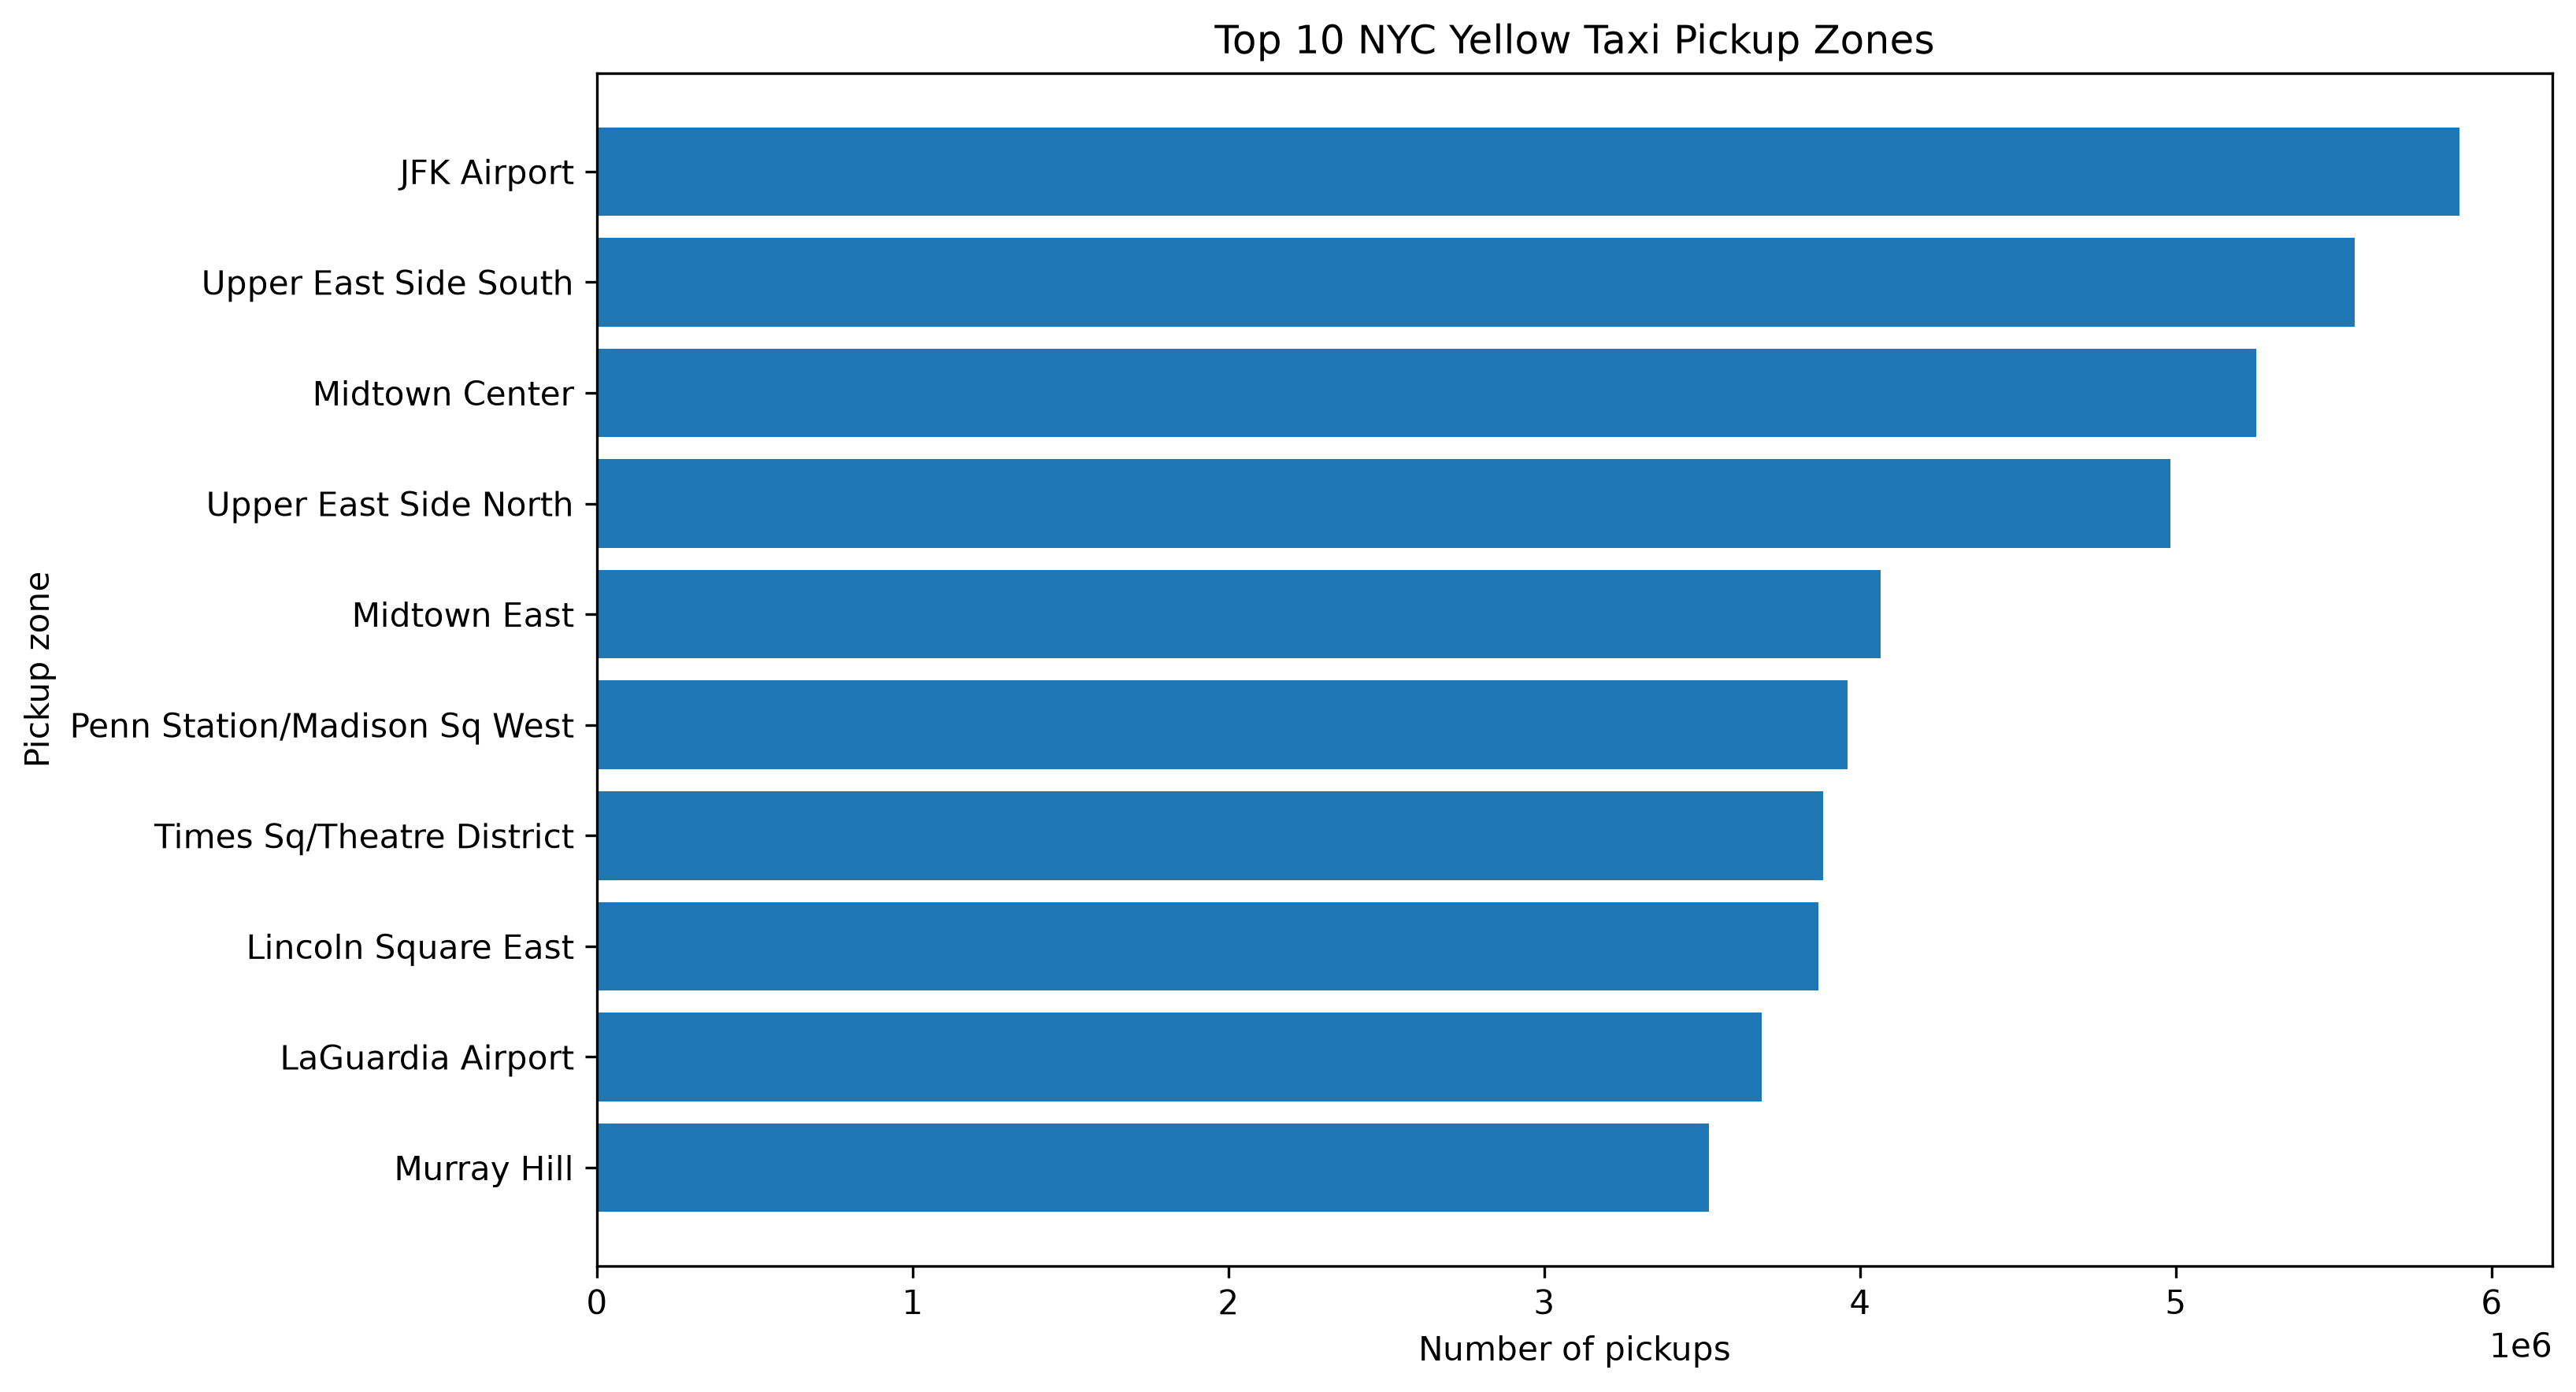
\includegraphics[width=0.82\textwidth]{figures/top_10_pickup_zones.png}
    \caption{Ten taxi zones with the highest pickup counts.}
\end{figure}

\subsection{Hourly Distribution}

Pickup demand changes considerably throughout the day. The lowest
number of pickups occurs at 04:00, with 681,496 trips. Activity
increases during the morning and reaches its maximum at 18:00,
with 8,457,664 pickups.

The period between 17:00 and 19:00 is particularly active, indicating
a strong concentration of trips in the late afternoon and early evening.

\begin{figure}[H]
    \centering
    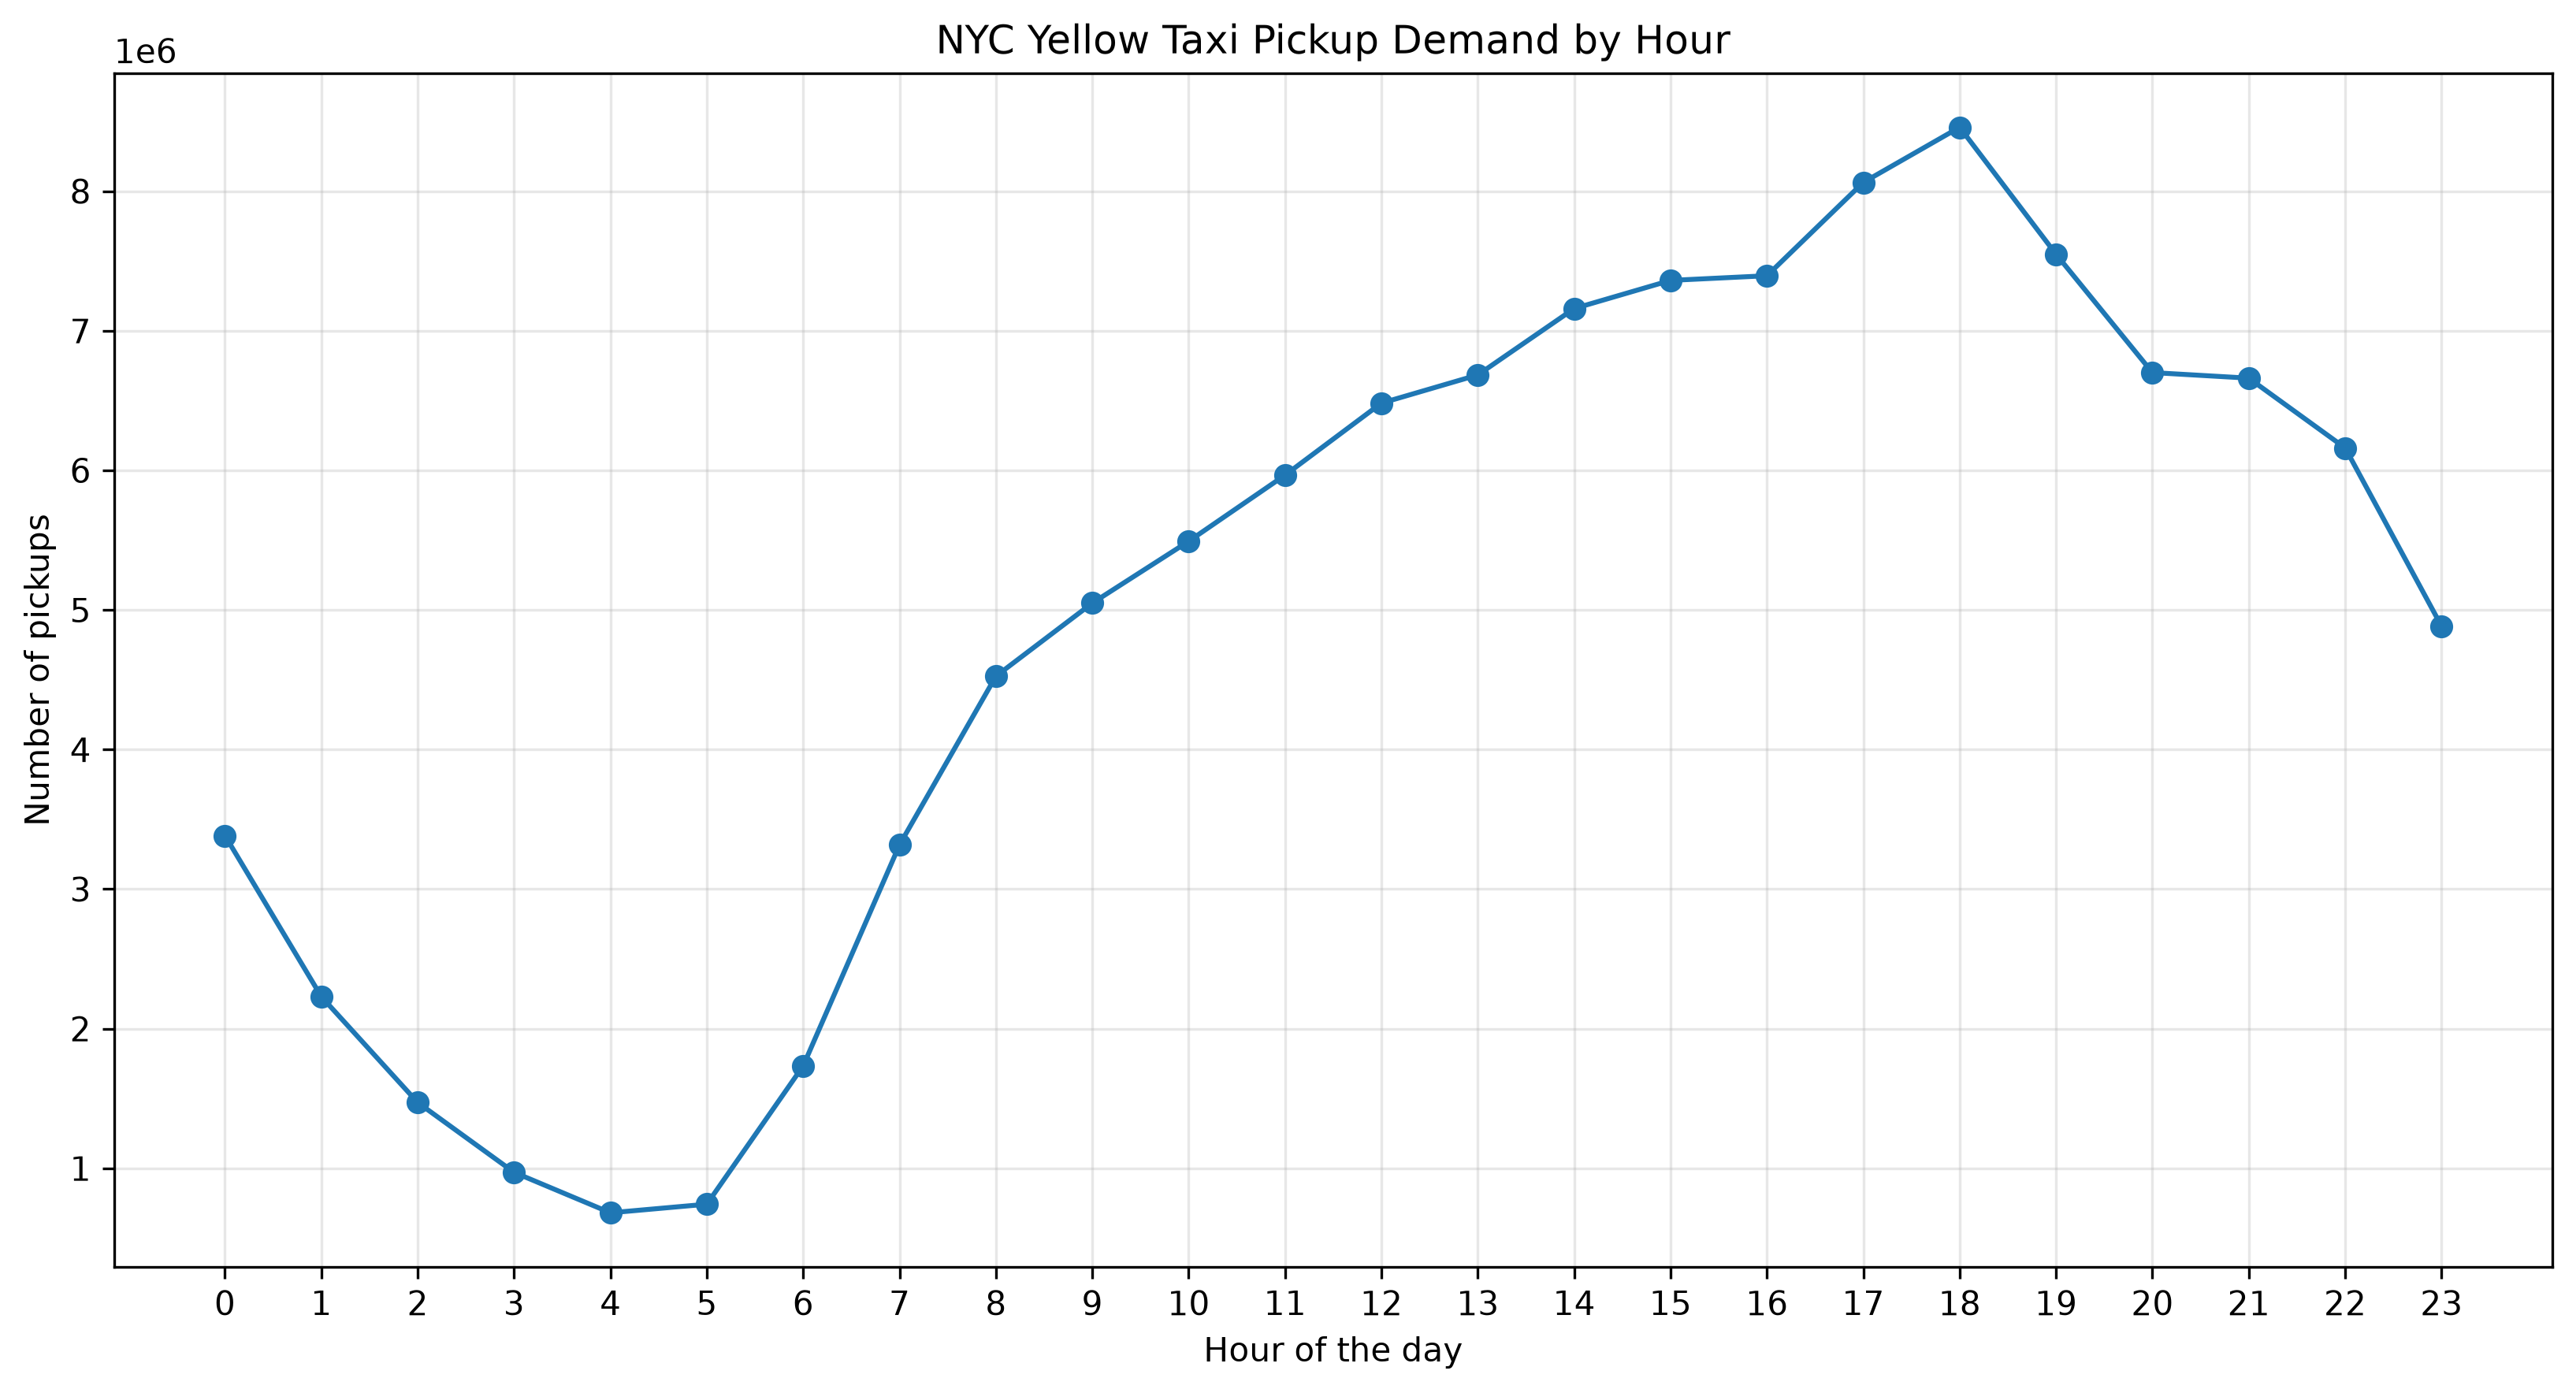
\includegraphics[width=0.82\textwidth]{figures/demand_by_hour.png}
    \caption{Pickup demand by hour of the day.}
\end{figure}

\subsection{Weekly Distribution}

Thursday is the busiest day, with 18,561,008 pickups, while Sunday
has the lowest count, with 14,899,572 pickups. Tuesday, Wednesday,
Friday, and Saturday also show relatively high activity compared
with Sunday and Monday.

\begin{figure}[H]
    \centering
    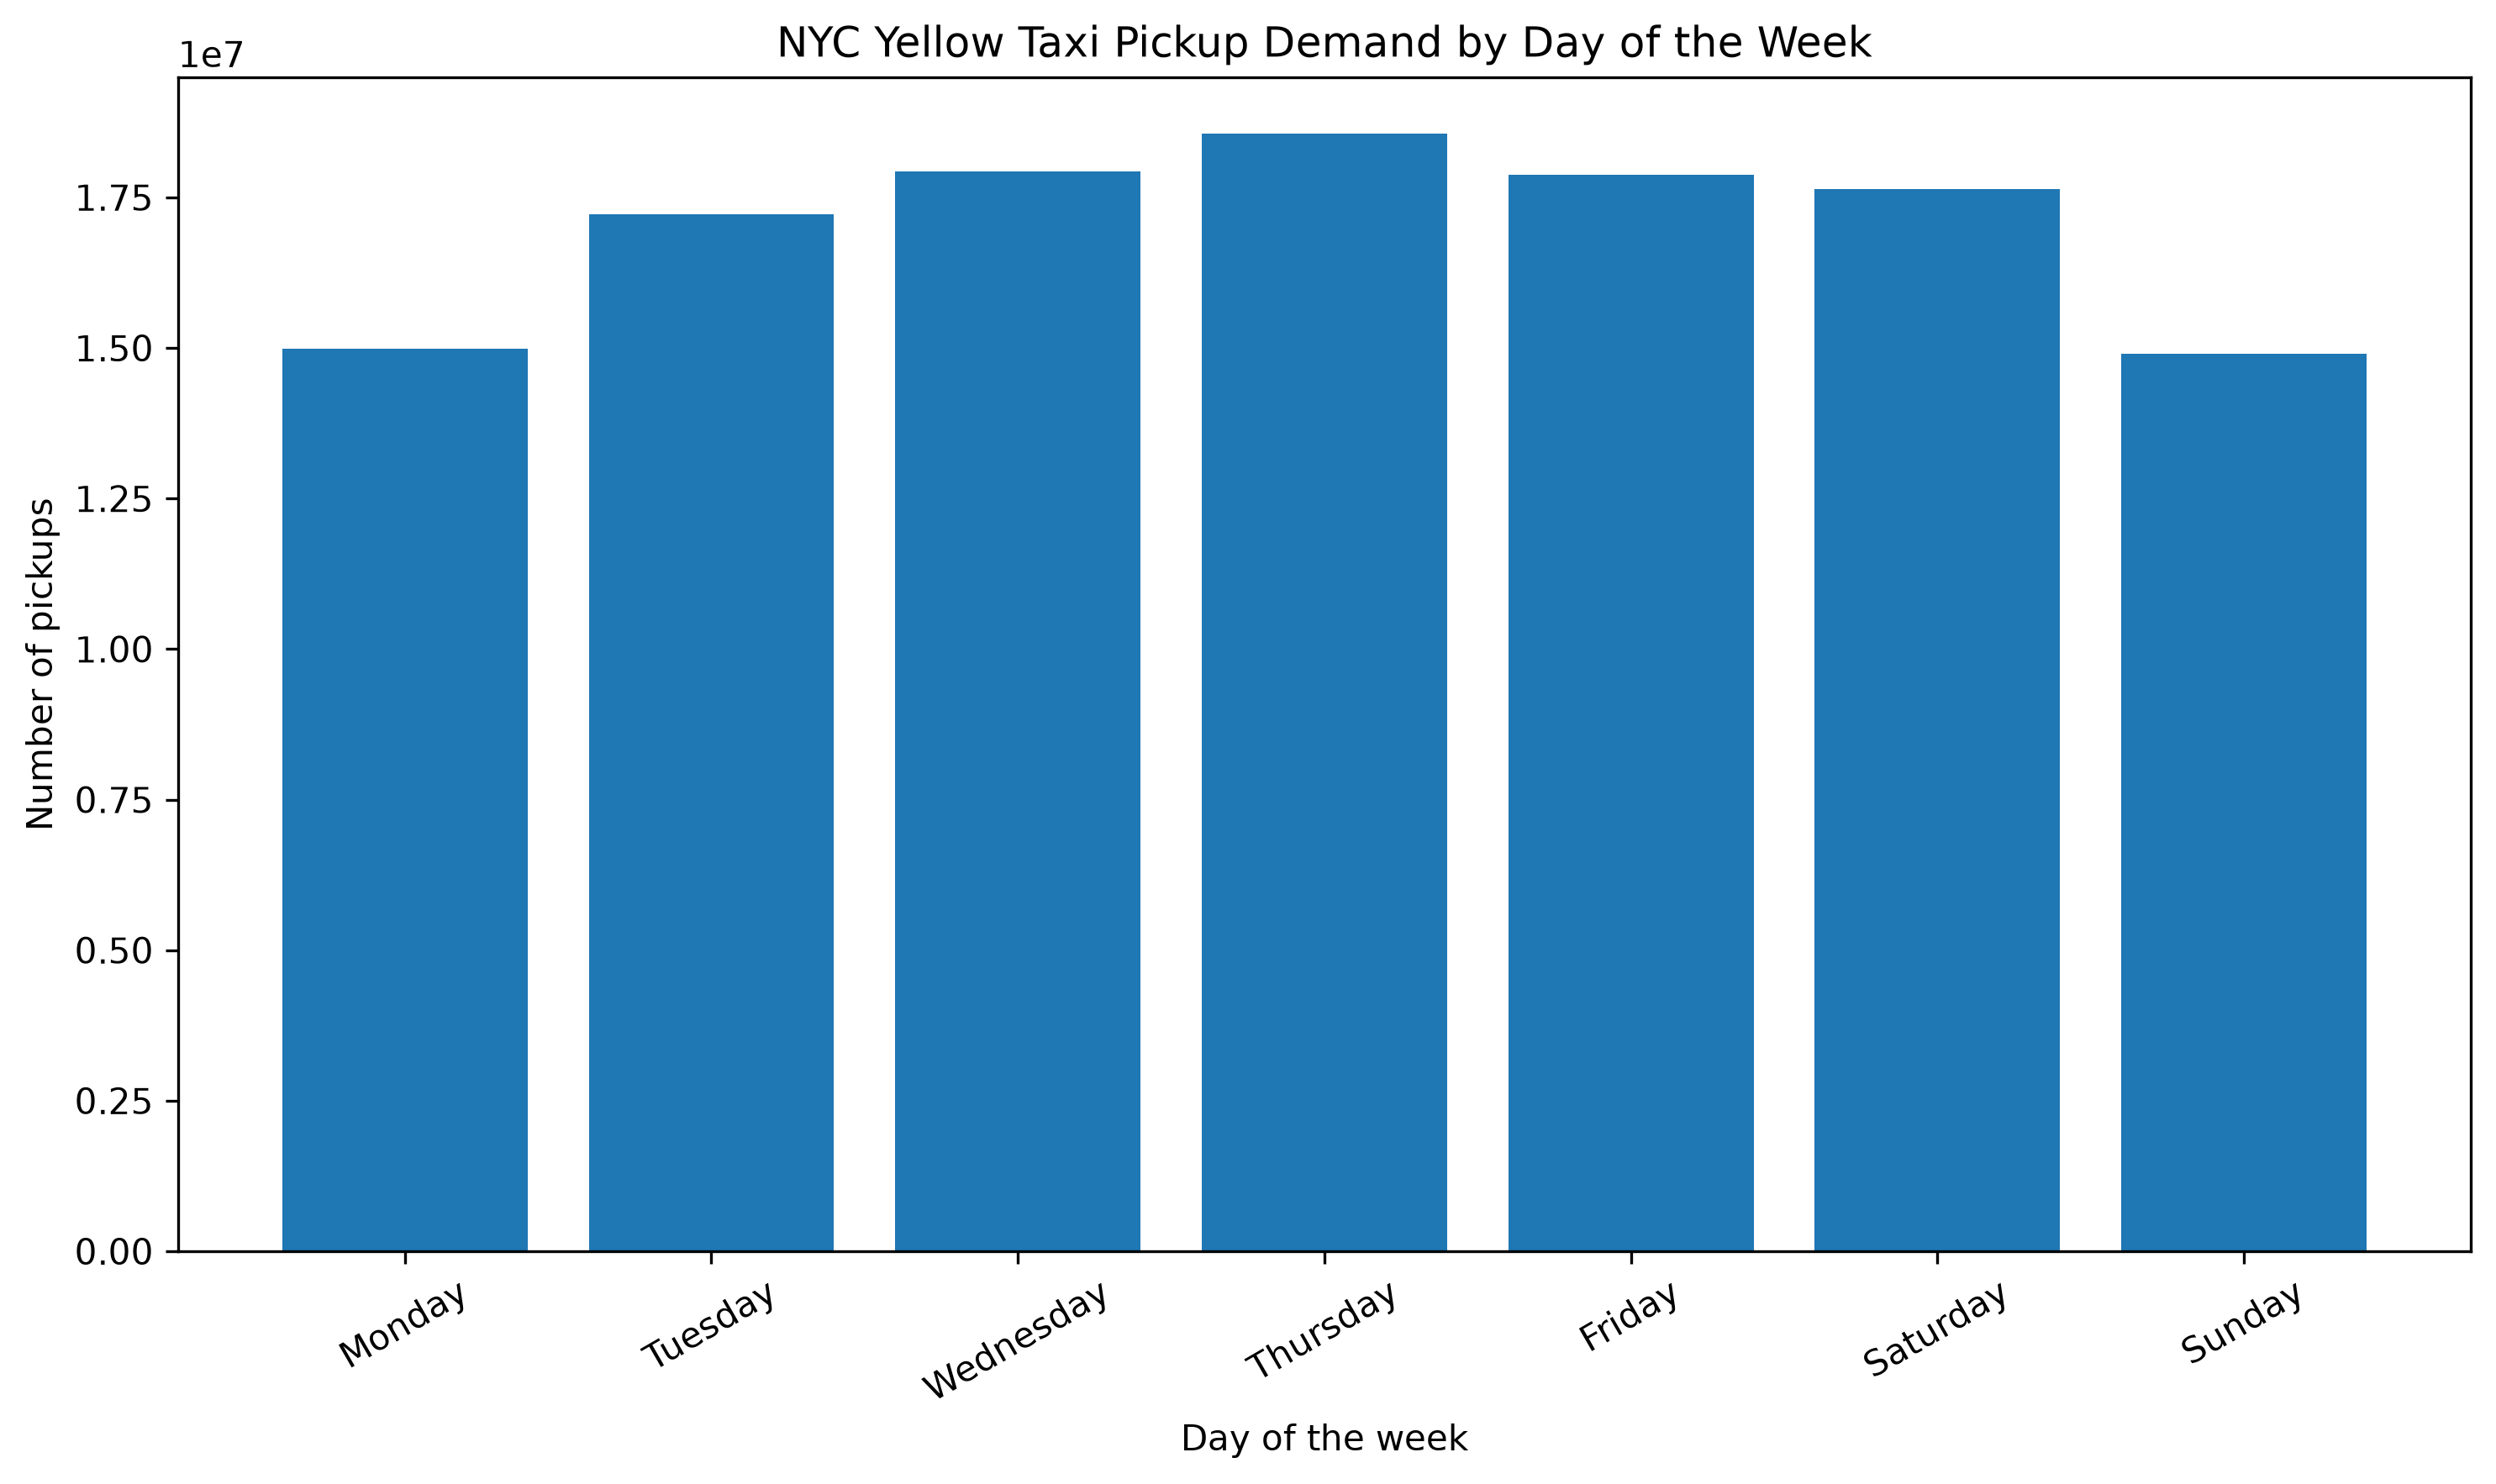
\includegraphics[width=0.82\textwidth]{figures/demand_by_day.png}
    \caption{Pickup demand by day of the week.}
\end{figure}

\section{Conclusion}

The analysis shows that yellow taxi pickup demand is not evenly
distributed across New York City or throughout the week. Airport
zones and central Manhattan locations record particularly high
pickup volumes. At the hourly level, demand reaches its maximum
at 18:00, while Thursday is the busiest day in the analysed period.

The results answer the Part 1 sub-question by identifying clear
spatial and temporal differences in pickup activity. The pipeline
also demonstrates how Apache Spark can process and aggregate a
large dataset while preserving reproducibility through scripted
acquisition, typed Parquet storage, cleaning, joining, and validation.

\end{document}
